% Bloch sphere -- standalone TikZ figure (compile with xelatex)
\documentclass[border=10pt]{standalone}
\usepackage{amsmath}
\usepackage{tikz}
\usetikzlibrary{arrows.meta}

% ---- colours -------------------------------------------------------------
\definecolor{spherefill}{RGB}{237,243,251}
\definecolor{sphereedge}{RGB}{ 62, 96,142}
\definecolor{gridcol}   {RGB}{158,173,193}
\definecolor{axiscol}   {RGB}{ 38, 44, 54}
\definecolor{statecol}  {RGB}{197, 48, 58}
\definecolor{anglecol}  {RGB}{ 22,113, 92}
\definecolor{helpcol}   {RGB}{112,122,136}

% ---- state to be drawn ---------------------------------------------------
\def\thetaval{55}   % polar angle
\def\phival{40}     % azimuthal angle

\begin{document}
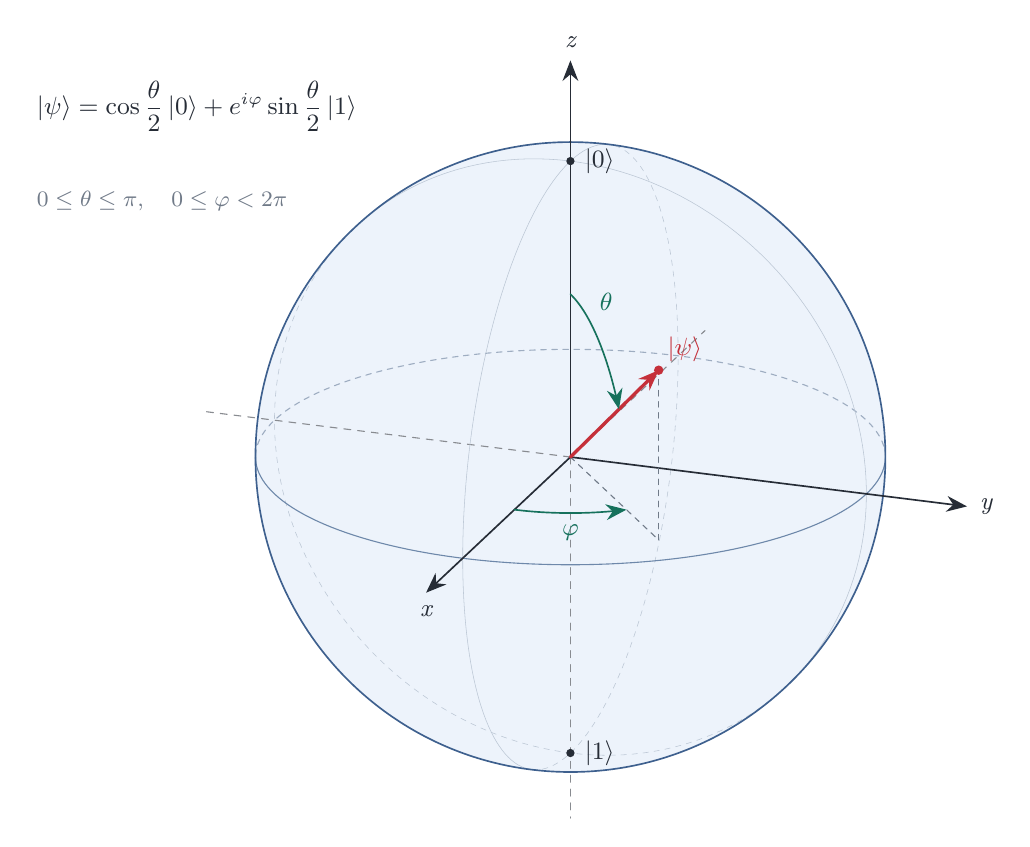
\begin{tikzpicture}[
  % orthographic projection: camera azimuth 20 deg, elevation 20 deg,
  % sphere radius = 4cm  (unit vectors below are already scaled by 4cm)
  x={(-1.36808cm,-1.28557cm)},
  y={( 3.75877cm,-0.46791cm)},
  z={( 0cm      , 3.75877cm)},
  >={Stealth[length=2.6mm,width=2.0mm]},
  line cap=round,line join=round,
  axislabel/.style={font=\small\itshape,text=axiscol},
  ketlabel/.style={font=\small,text=axiscol,inner sep=2pt}
]

% ---- sphere body ---------------------------------------------------------
\fill[spherefill] (0,0) circle[radius=4cm];

% ---- hidden (back) grid lines -------------------------------------------
\draw[gridcol,thin,dashed,dash pattern=on 2pt off 2pt]
  plot[domain=110:290,samples=90,variable=\t] ({cos(\t)},{sin(\t)},0);
\draw[gridcol!70,very thin,dashed,dash pattern=on 2pt off 2pt]
  plot[domain=158.8:338.8,samples=90,variable=\s] ({sin(\s)},0,{cos(\s)});
\draw[gridcol!70,very thin,dashed,dash pattern=on 2pt off 2pt]
  plot[domain=133.2:313.2,samples=90,variable=\s] (0,{sin(\s)},{cos(\s)});

% ---- negative half axes (behind the sphere) ------------------------------
\draw[axiscol!55,thin,dashed,dash pattern=on 2.5pt off 2.5pt] (0,0,0) -- (-1.25,0,0);
\draw[axiscol!55,thin,dashed,dash pattern=on 2.5pt off 2.5pt] (0,0,0) -- (0,-1.25,0);
\draw[axiscol!55,thin,dashed,dash pattern=on 2.5pt off 2.5pt] (0,0,0) -- (0,0,-1.22);

% ---- visible (front) grid lines -----------------------------------------
\draw[gridcol!70,very thin]
  plot[domain=-21.2:158.8,samples=90,variable=\s] ({sin(\s)},0,{cos(\s)});
\draw[gridcol!70,very thin]
  plot[domain=-46.8:133.2,samples=90,variable=\s] (0,{sin(\s)},{cos(\s)});
\draw[sphereedge!75,thin]
  plot[domain=-70:110,samples=90,variable=\t] ({cos(\t)},{sin(\t)},0);

% ---- silhouette ----------------------------------------------------------
\draw[sphereedge,semithick] (0,0) circle[radius=4cm];

% ---- positive half axes --------------------------------------------------
\draw[axiscol,semithick,->] (0,0,0) -- (1.34,0,0) node[axislabel,below=1pt] {x};
\draw[axiscol,semithick,->] (0,0,0) -- (0,1.34,0) node[axislabel,right=1pt] {y};
\draw[axiscol,semithick,->] (0,0,0) -- (0,0,1.34) node[axislabel,above=1pt] {z};

% ---- poles ---------------------------------------------------------------
\fill[axiscol] (0,0,1) circle[radius=1.5pt];
\fill[axiscol] (0,0,-1) circle[radius=1.5pt];
\node[ketlabel,anchor=west,xshift=3pt] at (0,0, 1) {$|0\rangle$};
\node[ketlabel,anchor=west,xshift=3pt] at (0,0,-1) {$|1\rangle$};

% ---- projection helpers --------------------------------------------------
\draw[helpcol,thin,dashed,dash pattern=on 2pt off 2pt]
  (0,0,0) -- ({sin(\thetaval)*cos(\phival)},{sin(\thetaval)*sin(\phival)},0);
\draw[helpcol,thin,dashed,dash pattern=on 2pt off 2pt]
  ({sin(\thetaval)*cos(\phival)},{sin(\thetaval)*sin(\phival)},0)
  -- ({sin(\thetaval)*cos(\phival)},{sin(\thetaval)*sin(\phival)},{cos(\thetaval)});

% ---- state vector --------------------------------------------------------
\draw[statecol,very thick,->]
  (0,0,0) -- ({sin(\thetaval)*cos(\phival)},{sin(\thetaval)*sin(\phival)},{cos(\thetaval)});
\fill[statecol]
  ({sin(\thetaval)*cos(\phival)},{sin(\thetaval)*sin(\phival)},{cos(\thetaval)})
  circle[radius=1.7pt];
\node[text=statecol,font=\small,anchor=south west,inner sep=3pt]
  at ({sin(\thetaval)*cos(\phival)},{sin(\thetaval)*sin(\phival)},{cos(\thetaval)})
  {$|\psi\rangle$};

% ---- polar angle theta (z axis -> state vector) --------------------------
\draw[anglecol,semithick,->]
  plot[domain=0:\thetaval,samples=40,variable=\s]
  ({0.55*sin(\s)*cos(\phival)},{0.55*sin(\s)*sin(\phival)},{0.55*cos(\s)});
\node[text=anglecol,font=\small]
  at ({0.72*sin(0.5*\thetaval)*cos(\phival)},
      {0.72*sin(0.5*\thetaval)*sin(\phival)},
      {0.72*cos(0.5*\thetaval)}) {$\theta$};

% ---- azimuthal angle phi (x axis -> projection) --------------------------
\draw[anglecol,semithick,->]
  plot[domain=0:\phival,samples=40,variable=\s] ({0.52*cos(\s)},{0.52*sin(\s)},0);
\node[text=anglecol,font=\small]
  at ({0.70*cos(0.5*\phival)},{0.70*sin(0.5*\phival)},0) {$\varphi$};

% ---- caption -------------------------------------------------------------
\node[anchor=west,text=axiscol,font=\small,align=left] at (-6.9cm,4.45cm)
  {$|\psi\rangle=\cos\dfrac{\theta}{2}\,|0\rangle
    +e^{i\varphi}\sin\dfrac{\theta}{2}\,|1\rangle$};
\node[anchor=west,text=helpcol,font=\footnotesize] at (-6.9cm,3.25cm)
  {$0\le\theta\le\pi,\quad 0\le\varphi<2\pi$};

\end{tikzpicture}
\end{document}
